\section{Ergebnisse}

\subsection{Einbinden von Nuitrack}
Nuitrack kann unter folgendem Link für alle Platformen runtergeladen werden: \href{https://github.com/3DiVi/nuitrack-sdk/blob/master/doc/Install.md}{\textbf{Nuitrack}}. \\ Die Software ist Platform unabhängig verfügbar und wird im gewünschten Folder auf der Festplatte installiert.

\subsubsection{Import Nuitrack Wrapper in Unity}
Unter folgendem Git Repo kann das Nuitrack Plugin runtergeladen werden: \href{https://github.com/3DiVi/nuitrack-sdk/blob/master/Unity3D/NuitrackSDK.unitypackage}{\textbf{Nuitrack Unity Plugin}}. Da dieses Plugin für verschiede Sensoren, also Kameras konfiguriert wurde, muss dann noch der Sensor spezifiziert werden. In meinem Projekt ist dies das Plugin für die IntelRealsense D435 Kamera.


\subsubsection{Skeleton Tracking mit NuitrackSDK}
Das Tutorial von Nuitrack ist meine Ausgangslage um eine Person zu tracken. Der Link führt zu diesem Tutorial: \href{https://github.com/3DiVi/nuitrack-sdk/blob/master/doc/Unity_Face_Tracking.md}{\textbf{Nuitrack Facetracking}}. \\ Das Tutorial ist gut beschrieben und lässt sich genau so umsetzen wie beschrieben.

\subsection{Virtuelle Szene in Unity}

\begin{figure}[H]
	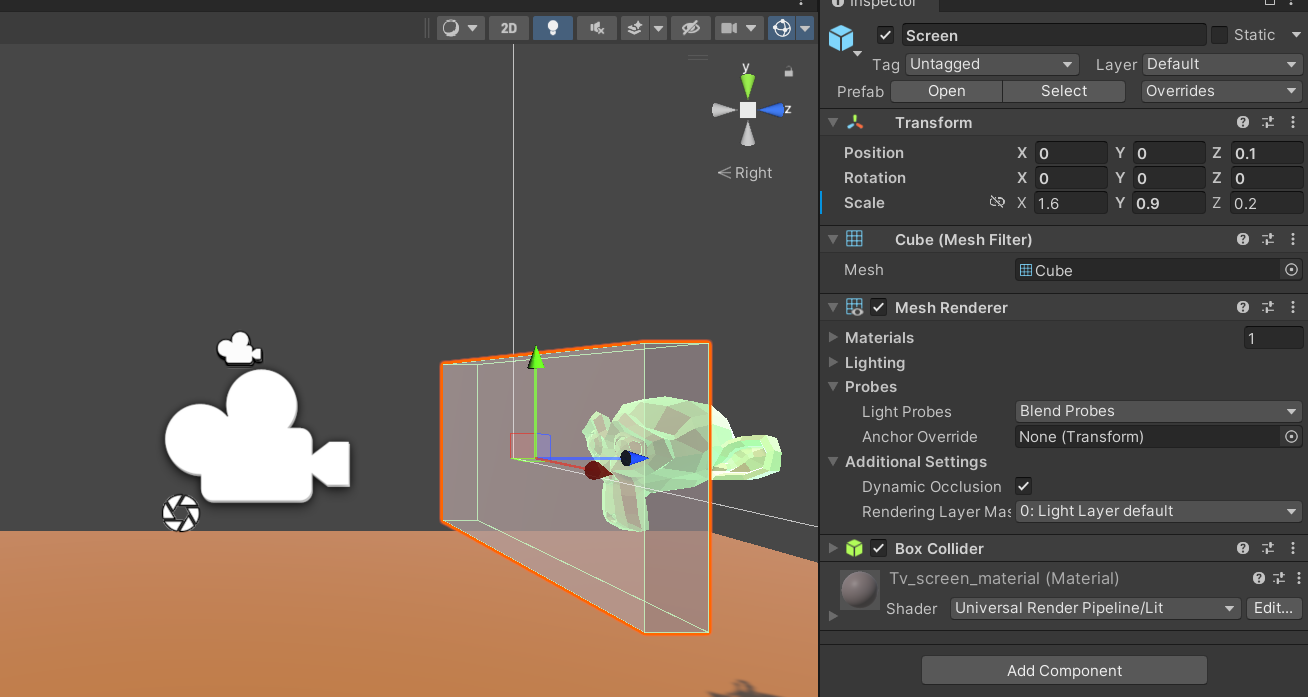
\includegraphics[width=1.0\linewidth]{Screen}
	\caption{Unity, Szene}
	\label{fig:Screen}
\end{figure}

In Unity baue ich die Szene so auf, dass die Render-Kamera in positiver z-Achse ausgerichtet ist. Anfangsposition der Render-Kamera ist (0, 0.2, -1.5). Den Screen welcher dann entzerrt werden soll, setze ich auf den Nullpunkt. Die Mitte vom Screen hat die Position (0, 0, 0).
Die Eckpunkte vom Screen haben die folgenden Positionen: 
P0(-0.8, -0.45)
P1( 0.8, -0.45)
P2( 0.8,  0.45)
P3(-0.8,  0.45)
Der Screen hat die Grösse 1600 x 900 mm. Dieser wird als schmaler Kubus dargestellt und transparent leicht grau eingefärbt, damit ich dann erkennen kann ob mein Rendern und Entzerren richtig funktioniert.
Die Main-Kamera setze ich als Referenz auf die Position der Render-Kamera. Dies damit ich eine Ansicht in der Szene bekomme. Die Main-Kamera zeigt dann die Szene und in der Game Ansicht zeigt die Render-Kamera den Output vom entzerrten Screen.  
Gut möglich, dass man dies auch mit weniger Kameras darstellen kann. \\ Figure~\ref{fig:Screen} zeigt den Aufbau der Szene mit dem grau eingefärbtem Screen und dessen Werte im Inspektor Fenster rechts daneben.

\subsection{Render Kamera zeigt Position vom Betrachter}
Die Render-Kamera wird als Referenz auf den obersten Knochen vom Skelett gemappt. Dieser oberste Knochen entspricht dem Kopf, genauer der Stirn.
Damit wird dann auch die Main-Kamera, welche die Render-Kamera referenziert auf den Kopf gemappt.

\subsection{Render Kamera zeigt RenderTexture}
Die Render-Kamera wird nun stets auf den Mittelpunkt vom Screen gerichtet. Der Output der Render-Kamera erzeugt dann eine RenderTexture der Grösse 750 x 750 Pixel. Je grösser die Anzahl Pixel, desto besser wird dann die Qualität vom Endbild.

\begin{figure}[H]
	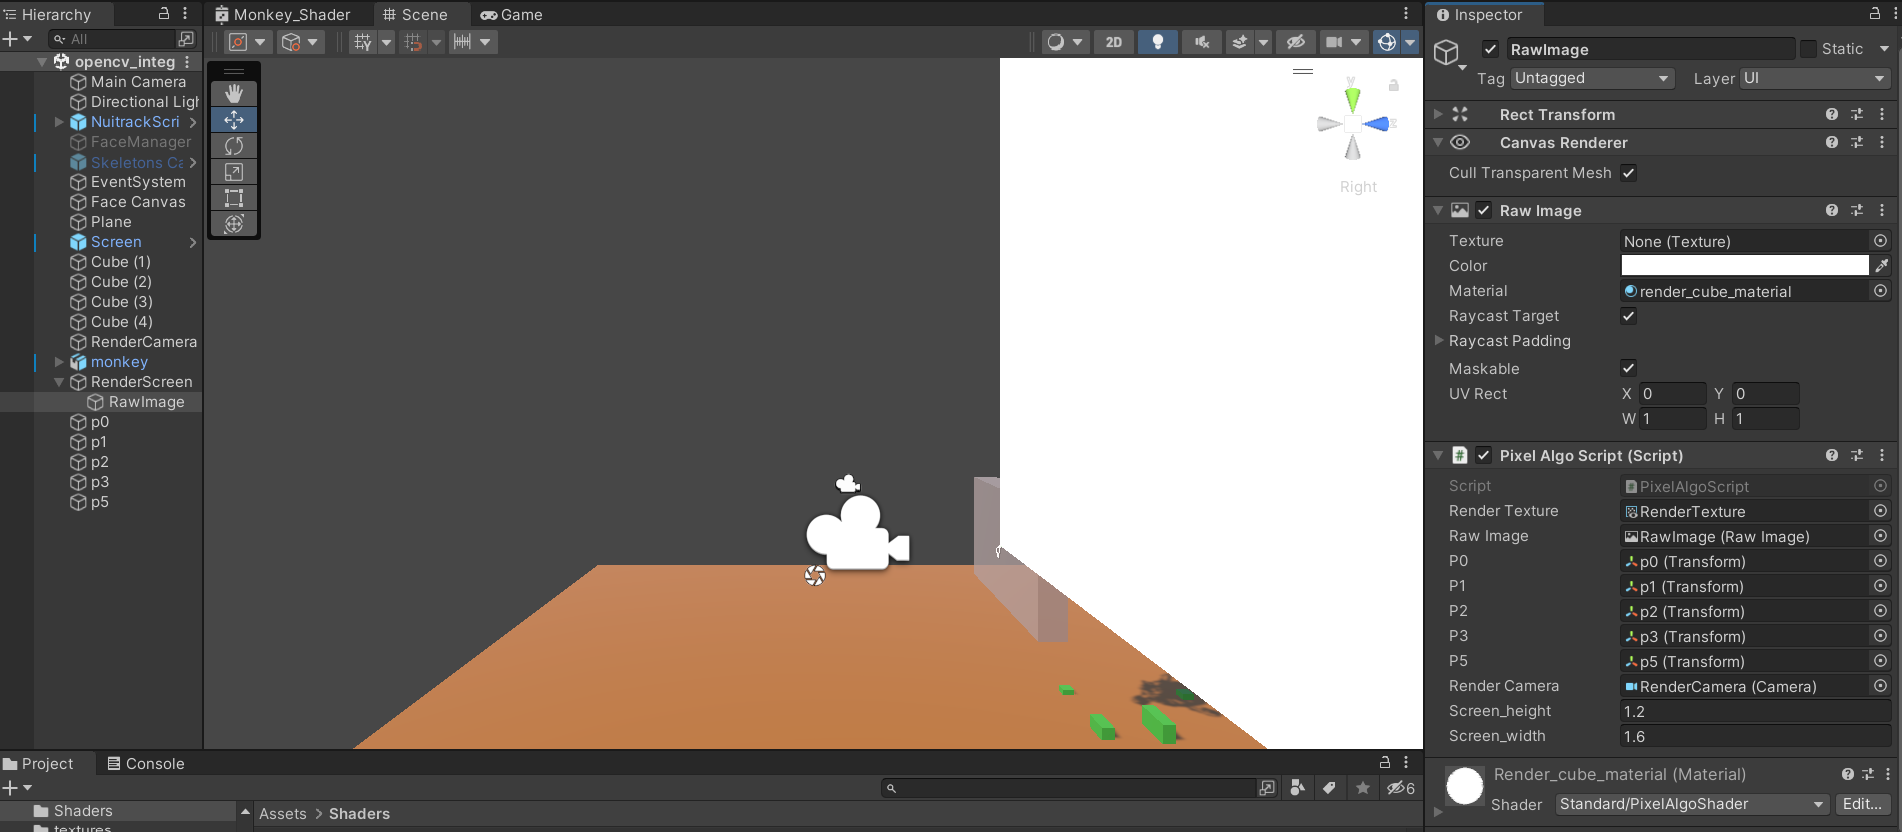
\includegraphics[width=1.0\linewidth]{RawImage}
	\caption{Unity, RawImage}
	\label{fig:Rawimage}
\end{figure}

Figure~\ref{fig:RawImage} zeigt das Output Bild, welches auf der weissen Ebene dargestellt wird. Diese entspricht nun dem Output Bild für den Screen und zeigt ein Format 16 : 9.


\subsection{Matrix Shader}
Im Netz habe ich einen Rotations Shader gefunden und versucht diesen so anzupassen, dass die Entzerrung gelingt. Leider ohne Erfolg. Das Probelm bei diesem Shader: Zwar funktioniert das Scaling und das Shearing, leider nicht aber die Translation.
Ich habe dann versucht eine Translation hinzuzufügen, was auch funktioniert hat.  

\begin{figure}[H]
	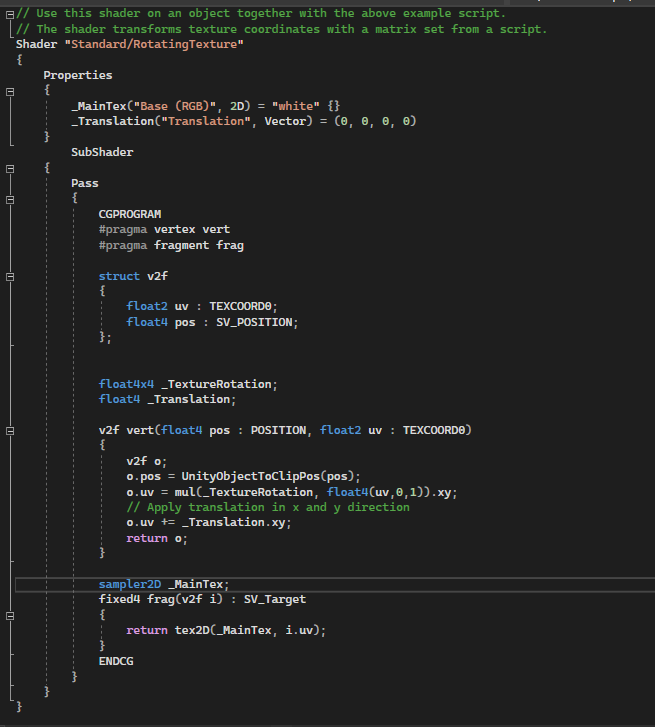
\includegraphics[width=0.8\linewidth]{Rotationsshader}
	\caption{Unity, MatrixShader}
	\label{fig:MatrixShader}
\end{figure}


Figure~\ref{fig:MatrixShader} zeigt den umgebauten Matrix-Shader mit einer Möglichkeit die x und y Koordinaten der Pixel zu verändern.
Leider weiss ich aber nicht, wie ich mit dieser Rotationsmatrix das Polygon selektieren soll und dann entzerrt darstellen.
Als Einstieg in die Unity Shader hat es trotzdem etwas geholfen, mehr aber auch nicht.

\subsection{Pixel Shader}
Damit ich diese Entzerrung vom Polygon machen kann, benötige ich einen Pixel-Shader. Oder einen Shader welcher die Maintexture ändert.
Ich erstelle nun so Schritt für Schritt einen Shader welcher als Parameter die Maintextur als Eingabewert hat. Und diese Maintexture dann im Shader jeweils angepasst wird. \\  Im Script wird in der Update Funktion für jedes Pixel der Farbwert gesetzt und am Ende die Textur dem Shader übergeben.


\begin{figure}[H]
	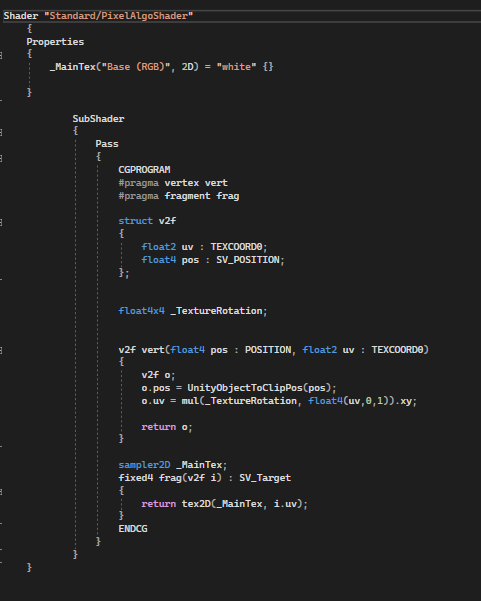
\includegraphics[width=0.8\linewidth]{PixelAlgoShader}
	\caption{Unity, Pixel-Shader}
	\label{fig:PixelShader}
\end{figure}

Figure~\ref{fig:PixelShader} zeigt den Shader, welcher die Texturen verändert, indem die Pixelwerte der Maintexture verändert werden.

\subsection{Homographie}
Unter dem folgenden Link habe ich ein Git Repo gefunden, welches die Homographie Matrix mit Gauss Elimination durchführt: 
\href{https://github.com/chiragraman/Unity3DProjectionMapping/blob/master/Assets/Scripts/Homography.cs}{\textbf{Homographie Matrix Berechnung}}.
Zuerst habe ich versucht die Entzerrung mit einer Homographie Matrix zu erreichen. Leider hat dies nur geklappt für die Ansicht ohne seitliche Verschiebung, also mit einem x-Wert von Null. Sobald ich etwas abweiche von dieser zentralen Position, zeigt sich ein Shearing im Output Bild, welches sich auch noch anders verhält, je nachdem ich in positiver x-Achse gehe oder in negativer x-Achse. 
Ich habe da länger darüber nachgedacht, meine Homographie Matrix mehrmals geprüft, fand aber nicht heraus was das Problem war. Komisch ja auch, dass es in zentraler Position den richtigen Output gab, bei seitlicher Verschiebung sich dann aber ein Shearing zeigt, welches mit grösserer Abweichung nach links oder rechts dann auch noch grösser wurde.
Somit brauche ich nun einen anderen Ansatz um die Entzerrung zu lösen.

\subsection{OpenCV}
OpenCV hat bereits Methoden, welche diese Entzerrung vornehmen. Das Plugin von OpenCV findet sich unter: \href{https://github.com/EnoxSoftware/OpenCVForUnity/tree/master/Assets/OpenCVForUnity}{\textbf{OpenCV Unity Plugin}}.
Die grösste Schwierigkeit ist bei OpenCV, dass Unity einen anderen Aufbau der Matrizen hat und dass OpenCV keine Textures kennt. 
Die grösste Schwierigkeit war dann zu merken, dass die Pixelwerte der Textures in OpenCV nicht einfach so auf der CPU verfügbar sind. Diese werden auf der GPU gespeichert und mössen dann exklusiv abgefragt werden.
Die Funktionen von OpenCV funktionieren tadellos. Damit die Entzerrung gelingt, gehe ich vom Zielbild aus und berechne die Perspektivische Matrix rückwärts vom Zielbild zum Inputbild, was dann dem Inversen der Perspektivischen Matrix entspricht. 
Nun wird diese Matrix auf jedes Pixel des Zielbildes angewendet und so den Farbwert an der entsprechenden Stelle im Inputbild geholt. 
Da diese Operation mit der Anzahl Pixel steigt, habe ich hier ein Format vom Zielbild 800 x 450 Pixel gewählt.

\begin{figure}[H]
	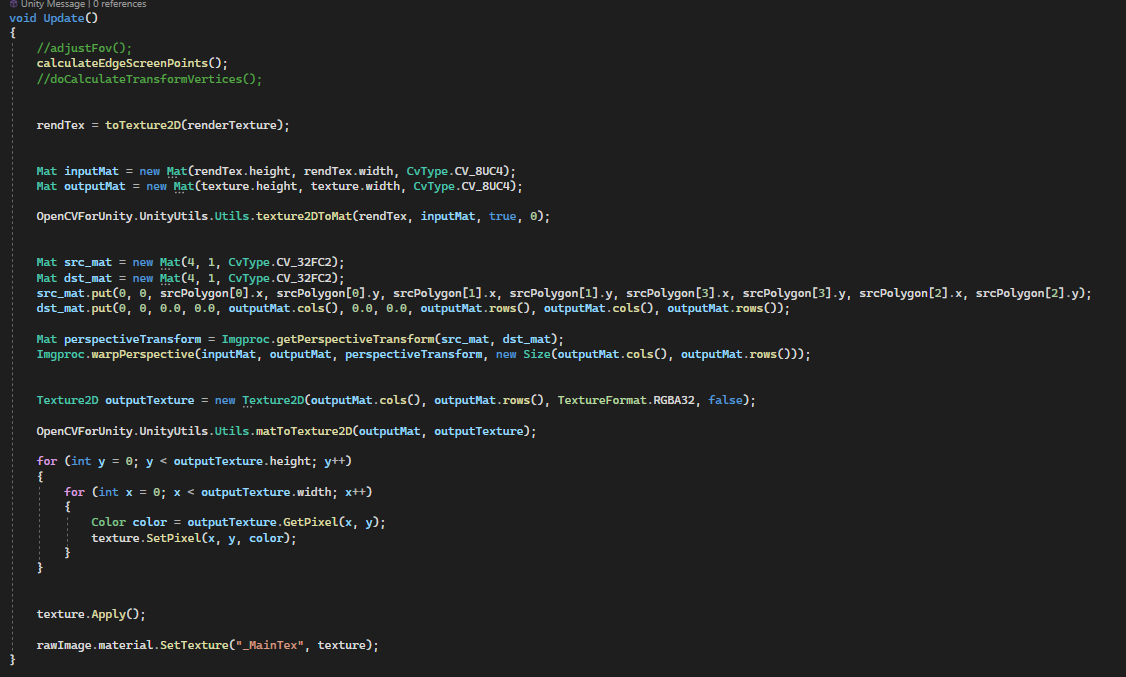
\includegraphics[width=1.0\linewidth]{OpenCV}
	\caption{Unity, OpenCV}
	\label{fig:OpenCV}
\end{figure}

In Figure~\ref{fig:OpenCV} zeigt sich diese Problematik. Die Textures werden in OpenCV Mat, also Matrizen umgewandelt. Die wichtigen Methoden von OpenCV sind dann: \\  
Mat perspectiveTransform = Imgproc.getPerspectiveTransform(srcMat, dstMat); \\
In getPerspectiveTransform wird die Homographie-Matrix anhand der vier Quellpunkte und der vier Zielpunkte berechnet. Die andere wichtige Methode von OpenCV: \\ 
 Imgproc.warpPerspective(inputMat, outputMat, perspectiveTransform, new Size(outputMat.cols(), outputMat.rows())); \\ In dieser warpPerspective Methode passiert die Entzerrung. In outputMat ist dann die gewünschte, entzerrte Textur, aber noch nicht als Textur. Deshalb wird dann diese OpenCV Mat in eine Textur umgewandelt. \\ Damit überhaupt etwas angezeigt wird braucht es nun noch diese explizite Abfrage der Pixelwerte, welches im Code in der For Schleife passiert.  \\ Am Ende wird die neu generierte Textur dem Pixel-Shader übergeben. Dies passiert mit der letzten Zeile: \\
 rawImage.material.SetTexture(" MainTex", texture);

\subsection{Kameramodell}
Ich habe versucht mittels Kameramodell die Transformationsmatrix für die Eckpunkte vom Screen zu berechnen. Dazu braucht man den Viewport, die intrinsiche (Projektionsmatrix) und die extrinsische Kameramatrix (Viewmatrix). Da sich der Screen nicht verschiebt, braucht es die Modellmatrix nicht.

\begin{figure}[H]
	\includegraphics[width=1.0\linewidth]{KameraMatrix}
	\caption{Unity, Berechnung Kameramatrix}
	\label{fig:Berechnung Kameramatrix}
\end{figure}

\begin{figure}[H]
	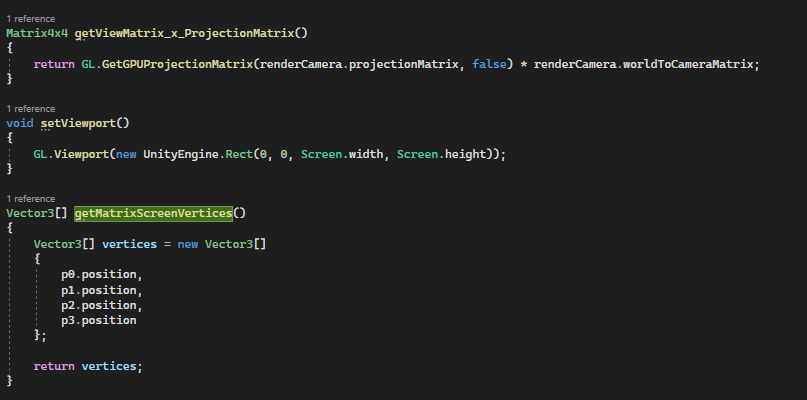
\includegraphics[width=1.0\linewidth]{Kameramatrix2}
	\caption{Unity, Methoden Kameramatrix}
	\label{fig:Kameramatrix Methoden}
\end{figure}

In Figure~\ref{fig:Berechnung Kameramatrix} versuche ich die Kamera-Matrix zu berechnen, wie bereits im Kapitel Kameramodell beschrieben. In Figure~\ref{fig:Berechnung Kameramatrix} verwende ich die Unity Methoden: GetGPUProjectionMatrix, welche mir eine resultierende Matrix aus Viewmatrix * Projectionmatrix berechnet. Nun fehlt mir noch die Viewportmatrix. Ich habe versucht diese Matrix in einem ersten Schritt mit GL.Viewport festzulegen und dann noch etwas anzupassen mit der Matrix clip-to-viewport-matrix. Leider ohne Erfolg. Deshalb habe ich mich dann für einen etwas vereinfachten Ansatz entschieden.

\subsection{Projektion der Eckpunkte auf der Zielebene}
Mein Ansatz den ich umgesetzt habe funktioniert wie folgt: 
Unity hat eine Funktion welche mir die Eckpunkte von der Clipping Ebene entsprechend dem z Wert herausscheibt. Siehe Figure~\ref{fig:ViewportToWorldPoin}

\begin{figure}[H]
	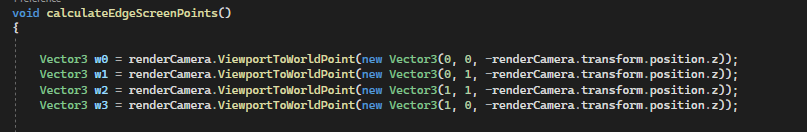
\includegraphics[width=1.0\linewidth]{ViewportToWorldPoint}
	\caption{Unity, Methode ViewportToWorldPoint}
	\label{fig:ViewportToWorldPoint}
\end{figure}

\begin{figure}[H]
	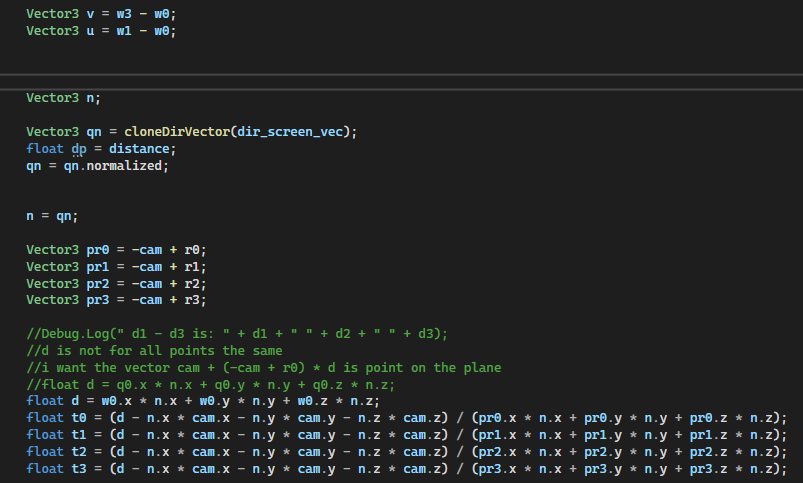
\includegraphics[width=1.0\linewidth]{Ebene}
	\caption{Unity, Ebene}
	\label{fig:Ebene}
\end{figure}

\begin{figure}[H]
	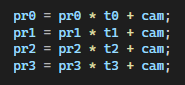
\includegraphics[width=1.0\linewidth]{Projektionsvektor}
	\caption{Unity, Projektionsvektoren}
	\label{fig:Projektionsvektoren}
\end{figure}


Ich wähle diese Ebene durch den Nullpunkt, auf welchen sich die Render-Kamera immer richtet. Die Berechnung der Ebene ist in der Abbildung Figure~\ref{fig:Ebene} dargestellt.\\
Nun projeziere ich die Eckpunkte vom Screen in der Verlängerung von der Render-Kamera durch die Eckpunkte. Die Berechnung dieser perspektivischen Vektoren in Richtung Eckpunkte vom Screen ist in der Abbildung  Figure~\ref{fig:Projektionsvektoren} dargestellt. Die Schnittpunkte mit der Ebene müssen nun nur noch relativ zu den Ecken der Clipping Ebene berechnet werden. Siehe untenstehende Graphik. Figure~\ref{fig:Eckpunkte} \\ Eigentlich hat auch der Richtungsvektor in y-Richtung eine x-Komponente, aber nur, wenn der Richtungsvektor in x-Richtung eine y-Komponente hat. Zur Vereinfachung nehme ich an, dass die Kamera horizontal ausgerichtet ist und dann wird dieser y-Anteil in x-Richtung gleich Null.

\begin{figure}[H]
	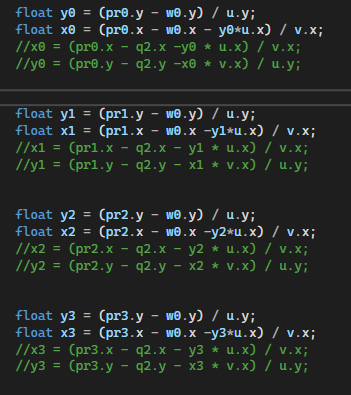
\includegraphics[width=1.0\linewidth]{Eckpunkte}
	\caption{Unity, Eckpunkte vom Screen}
	\label{fig:Eckpunkte}
\end{figure}






